\documentclass[10pt,letter]{article}
	% basic article document class
	% use percent signs to make comments to yourself -- they will not show up.

\usepackage{amsmath}
\usepackage{amssymb}
	% packages that allow mathematical formatting

\usepackage{graphicx}
	% package that allows you to include graphics

\usepackage{setspace}
	% package that allows you to change spacing

\onehalfspacing
	% text become 1.5 spaced

\usepackage{fullpage}
	% package that specifies normal margins
	
\usepackage[version=3]{mhchem} % Package for chemical equation typesetting
\usepackage{graphicx} % Required for the inclusion of images
\usepackage{natbib} % Required to change bibliography style to APA
\usepackage{amsmath} % Required for some math elements 
\usepackage{booktabs}
\usepackage{floatrow}
	

\begin{document}
	% line of code telling latex that your document is beginning


\title{CS 156 Problem Set 5}

\author{Christopher Zhen}

\date{Oct 31, 2016}
	% Note: when you omit this command, the current dateis automatically included
 
\maketitle 
	% tells latex to follow your header (e.g., title, author) commands.
	
\begin{align}
\textrm{Variants} & = 1500 \ (\frac{e^{-\lambda}\lambda ^x}{x!}) \\
& = 1500 \ (\frac{e^{-1} * 1 ^1}{1!}) \\
& = \frac{1500}{e} \\
& = 551.8
\end{align}

\begin{align}
\textrm{[E]} & = \textrm{[E]$_\textrm{T}$} - \textrm{[ES]} \\
\textrm{[ES]} & = \frac{\textrm{[E]$_\textrm{T}$}-\textrm{[ES]}}{K_\textrm{M}} \\
\textrm{[ES]} & = \frac{\textrm{[E]$_\textrm{T}$[S]}/K_\textrm{M}}{1+\textrm{[S]}/K_\textrm{M}} \\
\textrm{[ES]} & = \textrm{[E]$_\textrm{T}$} \frac{\textrm{[S]}}{\textrm{[S]}+K_\textrm{M}}
\end{align}

\begin{equation}
V_0 = k_2\textrm{[ES]}
\end{equation}

\begin{align}
V_0 & = k_2 \textrm{[E]$_\textrm{T}$} \frac{\textrm{[S]}}{\textrm{[S]}+K_\textrm{M}} \\
V_0 & = V_\textrm{max} \frac{\textrm{[S]}}{\textrm{[S]}+K_\textrm{M}} \\
\end{align}

\section*{Problem 1}

\textbf{(C)} - We can solve for the smallest possible possible value of N by solving the following equation:

\begin{align*}
\mathbb{E}_\mathcal{D}[E_\textrm{in}(\boldsymbol{w}_\textrm{ln})] & = \sigma^2(1 - \frac{d+1}{N}) \\
0.008 & = (0.1)^2(1 - \frac{(8)+1}{N}) \\
N & = 45
\end{align*}

So the lowest answer choice that satisfies the desired expected in-sample error is $N = 100$.

\section*{Problem 2}

\textbf{(D)} - To achieve the desired boundary, we can use the following formula of a hyperbola:

\begin{align*}
ax_1^2 - bx_2^2 & = 1 \\
ax_1^2 - bx_2^2 -1 & = 0 \\
\end{align*}

However, because this equation gives the opposite dichotomy as the one desired, we need to multiply everything by -1 to get:

\begin{align*}
-ax_1^2 + bx_2^2 +1 & = 0 \\
\end{align*}

Which matches with answer choice D.

%\begin{figure}[H]
%\begin{center}
%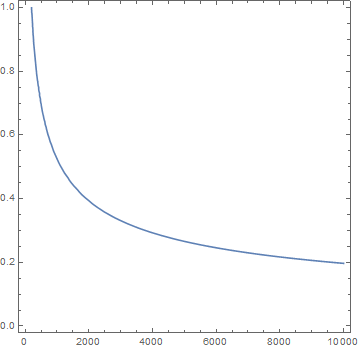
\includegraphics[width=0.5\textwidth]{2d.png}
%\caption{Table courtesy of the textbook %textit{Learning from Data}.}
%\label{2d}
%\end{center}
%\end{figure}

\section*{Problem 3} 

\textbf{(C)} - Since we know that $d_\textrm{vc} \leq \tilde{d} + 1$, we know that $d_\textrm{vc} < 15$.

\section*{Problem 4}

\textbf{(E)} - Using the chain rule and other differentiation rules, we find the derivative to match E.

\section*{Problem 5}

\textbf{(D)} - The code outputs 10 which matches answer choice D.

\section*{Problem 6}

\textbf{(E)} - The code outputs $(u,v) = [0.0447, 0.0239]$ which is closest to answer choice E.

\section*{Problem 7}

\textbf{(A)} - The code outputs 0.133 which is closest to A. This also makes sense because doing it this way should be slower than using gradient descent.

\section*{Problem 8}

\textbf{(E)} - The code outputs 0.189 which is closest to answer choice E. 

\section*{Problem 9}

\textbf{(A)} - The code outputs 264.2 which is closest to answer choice A.

\section*{Problem 10}

\textbf{(E)} - Since the step we want to take in PLA is $y_n \boldsymbol{x}_n$, our error function has to be of the form of $-y_n \boldsymbol{w}^\textrm{T}\boldsymbol{x}_n$. However, since PLA only cares about misclassified points, if a point is classified correctly, the error function should be 0, so we obtain the error function in answer choice E.

\end{document}
	% line of code telling latex that your document is ending. If you leave this out, you'll get an error
